\documentclass[10pt,letterpaper]{article}

\usepackage{cogsci}
\usepackage{pslatex}
\usepackage[nodoi]{apacite}
\usepackage{graphicx}
\usepackage[american]{babel}
\usepackage{amsmath}
\usepackage[section]{placeins}
\usepackage{enumitem}

\title{Children's Ability to Compute Implicatures in Simplified Tasks: \linebreak Availability of Alternatives and Prosodic Cues}
 
\author{{\large \bf Erica J. Yoon (ejyoon@stanford.edu)} \\
  Department of Psychology \\
  Stanford University
  \AND {\large \bf Charles Y. Wu (ywu15@wabash.edu)} \\
  Department of Psychology \\
  Wabash College
  \AND {\large \bf Michael C. Frank (mcfrank@stanford.edu)} \\
  Department of Psychology \\
  Stanford University}


\begin{document}

\maketitle


\begin{abstract}
Language comprehenders routinely make pragmatic inferences that go beyond the literal meanings of utterances. If A said ``I ate some of the cookies,'' B would probably infer that A ate `some \emph{but not all}' of the cookies. However, children often seem to fail to compute implicatures despite their early-emerging sensitivity to pragmatic cues. The current work sought to explore potential factors responsible for children's successes and failures in computing pragmatic inferences. In two Experiments, we used eye-tracking paradigm to test children's ability to compute implicatures when they have access to contextual alternatives to the target word (Experiment 1), and when they hear prosodic cues that emphasize the contrast between the target and alternative (Experiment 2). We found that young children successfully compute implicatures with access to contextual alternatives (4 years and older) and supportive prosodic cues (3 years and older). 

\textbf{Keywords:} 
Pragmatic cues; implicatures; cognitive development

\end{abstract}


\section{Introduction}

Language comprehension involves not only interpreting the literal meanings of words in utterances, but also understanding the communicative intentions behind what is said. Listeners often make inferences about \emph{pragmatic implicatures}, or speaker's implied meaning that goes beyond the conventional meaning of the utterance \cite{grice1975logic}. 

For example, if A says to B, ``Some of the students failed the test,'' B may infer that A intended to say ``Some, \emph{but not all}, of the students failed the test.'' That is, A's use of the term `some' \emph{implicates} that the stronger scalar alternative `all' is negated. These implicatures that involve scales built based on the knowledge of \emph{lexical} alternatives are called \emph{scalar implicatures} (\emph{SI}'s from here on).

Many studies have looked at the development of implicature understanding by testing adults' and children's ability to compute SI's. Whereas adults readily compute SI's, children tend to perform poorly on SI tasks (e.g., \citeNP{noveck2001children, papafragou2003scalar, huang2009semantic, barner2009finding, teresa2005children}). For example, in a context in which three out of three horses jumped over a fence and a puppet made a remark such as: e.g., ``some of the horses jumped over the fence,?? most of the adults rejected the statement as infelicitous, whereas close to 90\% of the children accepted it \cite{papafragou2003scalar}. % Huang and Snedeker here?

Children's failures on SI computation are surprising, given their early-emerging sensitivity to informativeness of utterances. For example, by 5 years of age, children are able to adjust informativeness of their own expressions depending on the listeners' knowledge \cite{matthews2006effect}; reward speakers based on the informativeness of their utterances \cite{katsos2011pragmatic}; and provide more information when disambiguation between potential referents is difficult \cite{matthews2012two}. At two years of age, when they are still too young to produce many utterances, children are able to assess informativeness of their own gestures \cite{o2001two}. Thus, even young children excel at assessing the informativeness of both their own and other people's utterances and communicative gestures. 

Based on the research on children?s sensitivity to communicative informativeness, it seems unlikely that children?s lack of pragmatic understanding is the cause of their failures on SI tasks. What factors are then responsible for their failures on SI computation? The current Experiments investigate two potential factors: availability of alternatives to the term offered; and cues that highlight the contrast between term offered and its alternatives. 

\subsection{Access to contextual alternatives}

Implicature computation involves generating and negating alternatives to a given term. For example, upon hearing `some,' the listener needs to generate a stronger alternative (in this case, `all') based on the lexical knowledge, and negate that alternative to compute the implicature.  

One potential cause of children's difficulty with previous SI tasks is their lack of access to lexical alternatives to the term offered \cite{barner2011accessing}. When adults hear `some,' they are able to generate the relevant scales and negate the stronger scalar alternative `all' to the term `some,' successfully computing implicatures. But for children, even if they know that there are alternatives to be negated, they may not be able to generate those relevant scalar alternatives. 

Indeed, there is evidence that children can compute ad-hoc implicatures, which depend on contextually-derived scales rather than lexically-derived ones \cite{stillerLLD} . Children saw three faces, one with glasses only, one with glasses and a top-hat, and one with none of the items. When children heard a puppet say: ``My friend has glasses,?? 3.5-year-old children and older chose the face with glasses only as the referent above chance. Thus, children were able to compute the implicature ``My friend has glasses, \emph{but not a top-hat}?? given the contextual access to the stronger alternative (face with glasses and top-hat) to be negated.

Even for this simplified task, however, children younger than 3.5 years still struggled to find the pragmatically correct referent. 




These findings lead to interesting questions to be explored about the developmental trajectories of implicature understanding. For example, \citeA{stillerLLD} showed children's final decisions for determining referents for utterances. But how are they making these decisions? Children younger than 3 still did not choose the pragmatically felicitous referent above chance in the modified task; what is it that contributes to the difference in performance by younger and older children? One possibility is that younger children rely more heavily on the literal meanings of utterances; another possibility is that there is an aspect of implicature tasks, unrelated to pragmatic understanding, that older children perform better compared to younger children, which consequently obscures younger children's ability for pragmatic inference. 

To answer these questions, it would be useful to look at children's real-time decision-making process, by using an eye-tracking paradigm. There are several advantages of using an eye-tracking paradigm to examine utterance processing; one can see how participants direct their eye gazes at each phase as an utterance is being produced, showing their judgment developing over time as compared to their one final judgment; also, eye gazes reflect a more implicit measure of comprehension than judgments made after conscious deliberation. Hence, eye-tracking paradigm is a useful tool in determining potential factors contributing to age differences in how fast children look toward inferential targets, and how much attention children give toward the targets at each phase of their utterance processing.

Experiment 1 explored children's on-line processing of ad-hoc implicatures through the eye-tracking paradigm. We sought to address three main goals: first, confirm whether, as Stiller et al.'s findings suggest, children younger than 5 years can compute implicatures; second, look at children's real-time decision-making process, as opposed to one-time judgments, for implicature computation; and third, identify potential factors that contribute to the developmental differences in implicature computation performance.

\section{Experiment 1}

\subsection{Method}

\subsubsection{Participants.}

Parents and their 2- to 5-year-old children visiting Children's Discovery Museum in San Jose, CA, were invited to participate in a short video study. The current sample comprised of children who were exposed to English at least 50\% of the time as indicated by their parents; individual trials with more than 50\% missing gaze data were excluded from analysis, and only those who completed at least 8 of 16 trials according to this criterion were included in the analysis. This left 93 out of initial 104 child participants whose data was analyzed: 24 2-year-olds (mean age = 2:6, range = 2:1-2:11, 10 female), 28 3-year-olds (mean age = 3:5, range = 3:1-3:11, 19 female), 24 4-year-olds (mean age = 4:6, range = 4:1-4:11, 13 female), 32 5-year-olds (mean age = 5:4, range = 5:1-5:9, 9 female). Children were given a sticker for participating in the study. 14 adult participants were undergraduate students recruited through Stanford Psychology credit pool.

\vspace{12pt}

\subsubsection{Stimuli and Design.}

On each trial, participants saw two images: a target and distractor, which could either be an item with a single feature (e.g., a plate with only a carrot or only a banana), or an item with double features (e.g., a plate with a carrot and a banana). Each trial contained three phases: in the initial phase (8.5 seconds), two images were presented in silence for two seconds, then a pre-recorded voice said a sentence (e.g., "Look at these plates. Elmo's plate has a carrot."). Then, in the anticipatory phase (1.5 seconds), a chime sound played to induce participants' anticipatory gaze. In the following feedback phase (1.5 seconds), a character appeared next to the target with an amusing sound effect. This was to keep the task engaging for child participants.

There were three types of test trials. In an \emph{inference} trial, the target item had a single feature (e.g., a carrot), and the distractor item had two features, one that was common with the target (e.g., a carrot) and the other feature that was unique (e.g., a banana). The test sentence named the feature that was common to the target and distractor. Thus, if participants understood that "Elmo's plate has a carrot" implicates "Elmo's plate has a carrot \emph{but not a banana}" given the context, they should look more toward the target than the distractor; otherwise, they should equally to both.

There were two additional trial types, with semantically unambiguous targets: \emph{control-double} trials looked identical to inference trials, but the target and distractor were switched, such that the double-feature item was the target and the single-feature item was the distractor, and the test sentence named the unique feature on the target. \emph{control-single} trials presented two items that each had a unique single feature, and either could be the target. Children saw 4 inference, 4 control-double, and 4 control-single trials; adults saw 6 inference, 6 control-double, and 12 control-single trials. 

% The two control trial types were included to prevent any potential confounds in how participants might determine referents; if only control-single trials were used as controls, then in the inference trials, participants might learn to look toward the target even before hearing the target word, from the statistical regularity that the single-feature item is always the target when two items in the trial are mismatched in the number of features. On the other hand, control-double trials did not match inference trials in terms of saliency of the target (a double-feature item is a more salient target than a single-feature item). Thus, both control trial types were used.

There were six sets of item and feature types, and the features were named with nouns found in MacArthur-Bates CDI. Two orders of the test trials were created, such that trial types and item types were counterbalanced and trial order was pseudo-randomized across the two orders.

\vspace{12pt}

\subsubsection{Procedure.}

Participants sat in a booster seat, approximately 60 cm away from the monitor of an SMI RED 120 Hz binocular remote eye-tracker. Participants were introduced to the task as watching a short video. The video began with a short Elmo video clip that lasted for 1-2 minutes, during which any necessary adjustments to the eye-tracker and participants' chair positions were made. The eye-tracker was then calibrated for each participant, using a 2-point calibration and validation of the calibration points. After calibration, participants were introduced to Sesame Street characters and were told `Today, [they] will show us lots of fun things. Are you ready? Let`s go!'

Following the introduction, participants saw two gaze-contingent practice trials, with unambiguous targets that differed from the test items. Then children watched 16 test trials and adults watched 24 test trials, as well as 4 filler photos of children playing and 2 Elmo video clips, presented at a pseudo-random points between test trials. The video lasted approximately 8 minutes.

\subsection{Results.}

For control trials, participants of all age groups looked toward the targets in both control-double and control-single trials reliably above chance (50\%; see Figure \ref{fig:age}). This shows that after they heard the unambiguous targets being named, children were able to correctly identify the targets. Some interesting patterns were found: first, there were age differences in the speed of looking at the target and the proportion of correct looking overall; these data are extension of the findings by \citeA{fernald1998rapid}, who found that children's efficiency of familiar word recognition over the second year; the current data show these gains in the efficiency seem to continue to increase through the childhood. Second, child participants looked more toward the target above chance even before the target word was produced. One plausible cause of this bias is the saliency of the target relative to the distractor: the target in a control-double trial was always visually more salient than the distractor, which might have attracted children's attention even before they heard it being named (see further discussion about the saliency effect in inference trials below). 

For inference trials, children older than 3 years showed robust looking to inferential targets. For example, upon hearing ``Bert's plate has a carrot,'' older children were able to identify the plate with only a carrot as the referent rather than the plate with a carrot and a banana. These results replicate Stiller et al.'s findings and suggest that children's inferential ability might have been obscured in previous SI tasks due to the unavailability of lexical alternatives to offered terms.

\begin{figure*}[t]
	\center{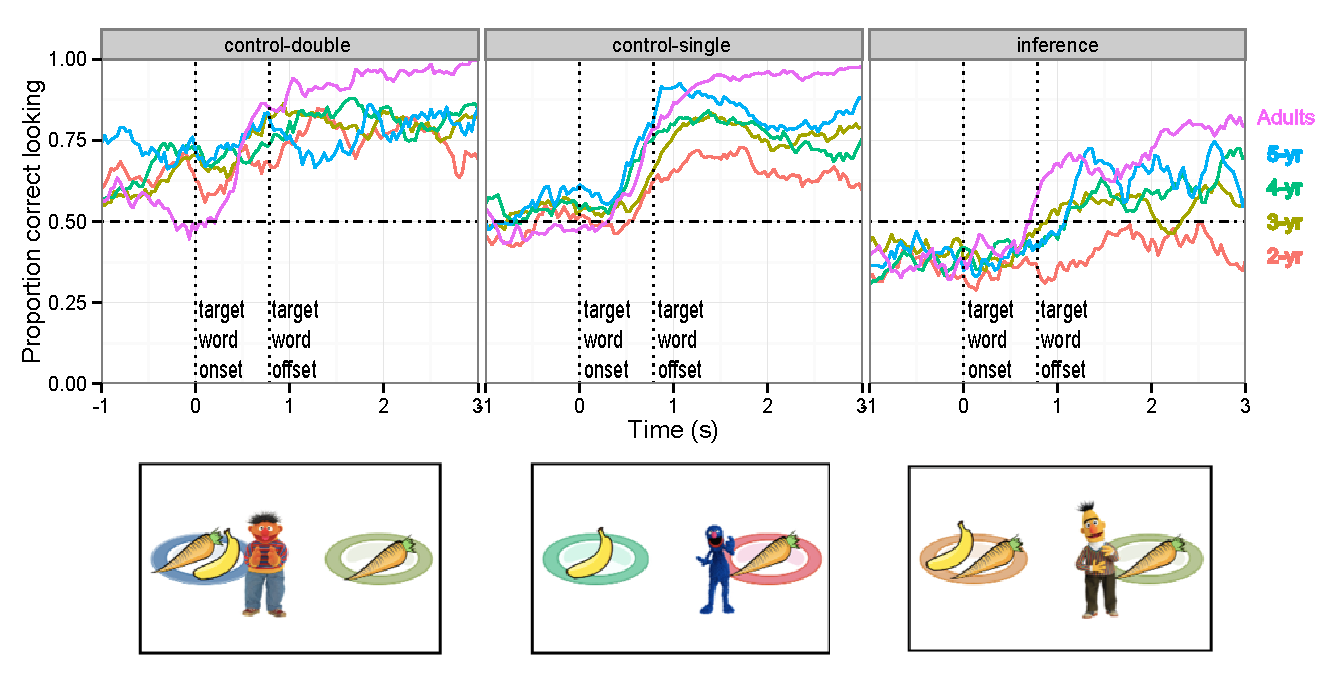
\includegraphics[width=\textwidth]{figures/140521-simpimp_age-edit.pdf}}
	\caption{\label{fig:age} Proportion of 2- to 5-year-old children and adults looking to the target image as the utterance unfolds. Time 0 represents the target noun onset. Proportion correct looking is defined by looks to the target divided by the total looks to both the target and the distractor.}
\end{figure*}

 Also, there were clear developmental trajectories looking to the inferential target increased with age. A linear mixed-effects model analyzed the effects of trial type, age group (as continuous), and time window (early: 1 s before noun onset - 1 s after noun onset;  late: 1 s - 3 s after noun onset) on the proportion of children looking to the target (see Table\ref{fig:table}). Results of this model indicate a significant interaction between the inference trial type and time window, such that children looked more toward the inferential target during the late window than during the early window. Also, there was a significant interaction between the inference trial type, age group, and time window, such that older children looked more toward the inferential target during the late window compared to younger children.

\begin{table}
\begin{center} 
\caption{\label{fig:table} Coefficient estimates from mixed-effects models predicting proportion of looks to target}
\includegraphics[width=3.5in]{figures/table.pdf}
\end{center} 
\end{table}

One possible factor besides implicature computation that could have affected children's judgments is learning effect: participants might have learned to locate the inferential targets from the feedback that showed them the target. If so, there should have been an order effect and participants should have improved in later trials, especially for inference trials if children failed to compute implicatures and had to rely on the feedback to figure out the referents; however, analyses revealed no order effect for any of the trial types (\emph{t} = .3).  

There were two additional interesting patterns revealed in the data: first, looks to the target were slower and overall lower in proportion in inference trials compared to both control trial types across all age groups. switches to targets from initial looks to distractors were slower for inferential than control targets (Figure \ref{fig:rt}). This suggests that implicatures are generally slower and harder to process compared to the unambiguous semantic meanings, regardless of the participants' age. Second, the two-year-olds' looking at the target was below chance, rather than at chance, which means they were looking significantly more at distractors than targets. Hence, two-year-olds did not seem to consider both the inferential targets and distractors as equally likely referents based on the literal meaning of the utterance; rather, the distractors attracted children's attention away from the target. 

\begin{figure}
\begin{center} 
\includegraphics[width=3.5in]{figures/150116-0-rt_age.pdf}
\caption{\label{fig:rt} Average reaction times for first switches to target in trials in which participants were looking at the distractor (and not the target) at the target word onset.}
\end{center} 
\end{figure}

To look more closely participants' eye gaze shift patterns in the inference trials, participants' switches in looking were examined (a method first introduced by \citeA{fernald2008looking}; see Figure \ref{fig:onset}).  For each age group, trials were divided into two groups: trials in which participants were initially looking at the distractor at the noun onset, and trials in which participants were initially looking at the target.  If participants computed the implicature, then distractor-initial group should increase their looking to the target, whereas target-initial group should continue to remain looking to the target. 

\begin{figure}
\begin{center} 
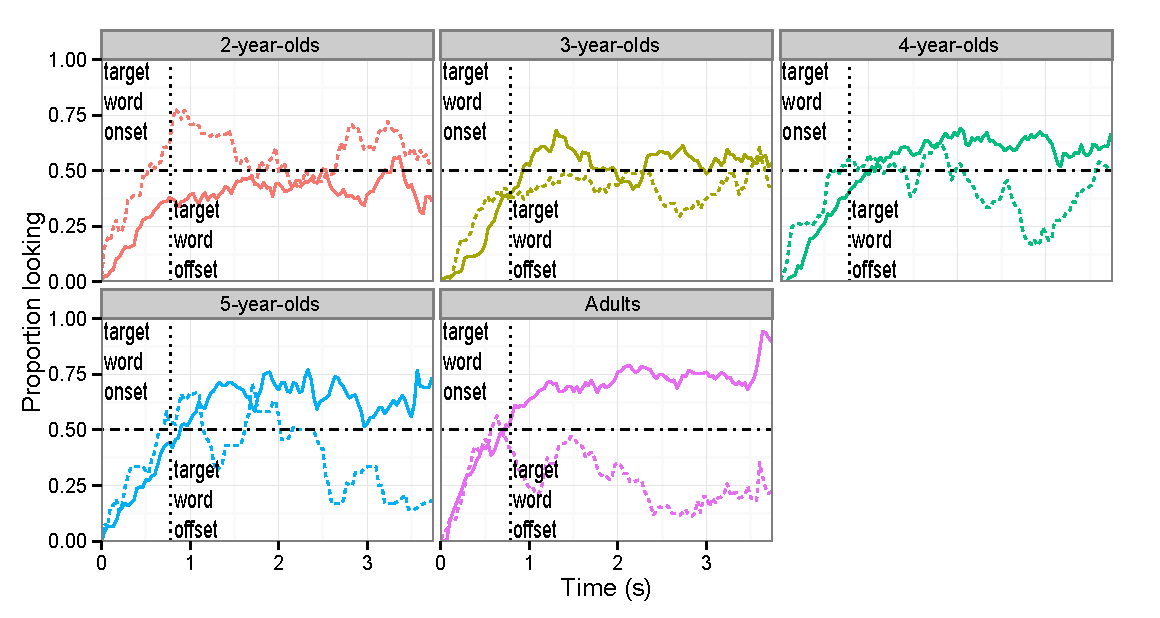
\includegraphics[width=3.5in]{figures/140521-simpimp_age_targAtOnset-edit.pdf}
\caption{\label{fig:onset} Looking to the target as a proportion of looking to the target and distractor across trial types. Children heard a sentence like ``Elmo's plate has a carrot (target word)'' then received feedback indicating the correct referent (i.e., characters? appearance next to the target item) 4 seconds after the target word onset.}
\end{center} 
\end{figure}

Current findings show that adults and children of 3 years and above follow these predictions: switch looks to the target after initial look at the distractor shoot up above chance after the target word has been produced. However, 2-year-olds actually show the opposite pattern: those who initially look at the target tend to switch and look at the distractor, whereas those who initially look at the distractor fail to switch to the target above chance. 

One possible cause of this pattern is the differential saliency of the target and distractor, except in inference trials the relative saliency is switched between the target and distractor: the distractor is always perceptually and conceptually more salient, because it contains an extra item. Thus, the listener has to overcome the greater saliency of the distractor and devote more attention to the target based on the pragmatic inference, requiring his or her inhibitory control. 

Inhibitory control is difficult for children and continues to develop through childhood, as shown in the literature on executive control \cite{davidson2006development, gerardi2000sensitivity}. A number of studies also found that children's lack of inhibitory control might affect recognition of newly learned words \cite{yurovskybeyond} and processing of negative utterances \cite{nordmeyer2013measuring}. It is plausible that similar inhibitory control constraints hindered younger children's correct looking to the inferential targets on the current work. 

Given this potential issue with inhibitory control for younger children, the current results have at least two different interpretations, both of which posit that older children have good pragmatic understanding and they are also better at inhibitory control than younger children, but make different predictions about younger children's pragmatic understanding: younger children might have poorer pragmatic understanding compared to older children, and they theoretically consider both objects as equally likely referents, but pay more attention to the more salient object. On the other hand, in another interpretation, both younger and older children might have good pragmatic skills, but younger children's attention to the more salient object is caused by their lack of inhibitory control.

In Experiment 2 we looked more closely at the effect of saliency gap between target and distractor in inference and control-double trials. In addition to trials in which single-feature and double-feature items were presented together, we added trials that presented single-feature and triple-feature items side-by-side. If inhibitory demands are present and affect implicature processing, we should see greater performance gap between control trials and inference trials in the newly added trials. 

Another issue that we were interested in exploring was the discrepancies in children's performances as captured by different methodologies. Even though we replicated \citeA{stillerLLD}`s findings that children of 4 years and above successfully compute implicatures, 4-year-olds in \citeA{stillerLLD} identified the pragmatically correct referent with close to 75\% accuracy rate, even though their paradigm had an additional foil besides a distractor, whereas 4-year-olds in our Experiment 1 had accuracy rate closer to 60\%. If the new paradigm is valid, this difference should arise not from linguistic phenomena of our interest but due to the different natures of the task: explicit choice-making paradigm such as the one used by \citeA{stillerLLD} should yield higher accuracy rates compared to implicit eye-tracking measure, during which participants make more spontaneous and unintended shifts in gazes. Experiment 2 addresses this concern by using forced-choice selection paradigm, in which participants mark their response explicitly; if our assumption about the validity of the measure is correct, Experiment 2 should yield results that are overall closer to \citeA{stillerLLD}'s findings; but at the same time, we predict some differences due to the varying saliency gap between items. 

\section{Experiment 2}

\subsection{Method}

\subsubsection{Participants.}

Participants were recruited from Children's Discovery museum in San Jose as in Experiment 1, and from the Bing Nursery School at Stanford University. For Experiment 2, we recruited 3- to 5-year-old children. The final sample consisted of X 3-year olds (X female), X 4-year olds (x female), and X 5-year olds (x female).

% As of 1/16/2015: 17 3y, 12 4y, 8 5y

\subsubsection{Stimuli and Design.}

Stimuli for test and practice trials were identical to those in Experiment 1, except in the following ways: the images of target and distractor were presented on an iPad tablet as cropped images on a black background. Once participants indicate their choice by touching one of the two images on screen, the image became outlined in green, and the images faded and disappeared, after which the images for the next trial showed up. There were no video clip or introduction video at the beginning, and no filler trials in between.

\subsubsection{Procedure.}

Participants sat at a table at approximately 20 cm distance from the iPad tablet. First they were introduced to the touch screen with a simple task of touching dots and smiley faces on screen to make them transform. Then the experimenter introduced a new ``game'' and explained the test trials that would follow. For the two following practice trials, experimenter scaffolded if the participant needed assistance; once test trials started, experimenter maintained minimal interaction with the participant. Participants saw 16 test trials: 4 inference and 4 control-double trials, half of which presented triple-feature items instead of double-feature items; and 8 control-single trials, half of which presented two double-feature items (the second feature was an extra common feature across both items) instead of two single-feature items.

\subsection{Results and Discussion.}

\begin{figure*}
	\center{\includegraphics[width=\textwidth]{figures/150116-scmN1-accuracy1.pdf}}
	\center{\includegraphics[width=\textwidth]{figures/150116-scmN1-accuracy.pdf}}
	\caption{\label{fig:mixnumAcc} Top: Accurate response rates for trial types and age groups. Bottom: Accurate response rates for trial types, number of features present and age groups.}
\end{figure*}

As for comparing different trial types, similar to what we found in Experiment 1, inference trials yielded lower accuracy rate compared to control trials.

Age differences in responses were also replicated: 5-year-olds had higher accuracy rates than 3-year-olds for inference trials.

This Experiment also provided a measure of methodological validity of the current paradigm. Results were closer to \citeA{stillerLLD} in that accuracy rates were much higher compared to eye-tracking. In fact 3-year-olds seem to perform better in this paradigm compared to \citeA{stillerLLD}, plausibly because the current task is easier with two instead of three items, and more engaging with touch-contingent visual and audio stimuli.

For the main question of interest for this Experiment: did varying the number of features have an effect on children's accuracy rate or reaction time to inference or control trials?

As for accuracy rate: yes, different number of features seem to affect target identification. But it is not the accuracy rate for inference trials that changes (decreases as saliency gap increases, as expected); it is the accuracy rate for control-double trials that \emph{increases} as their targets gain saliency. Thus, the relative performance gap between control-double trials and inference trials seem to be driven by more attentional resources being spent on the distractor, not by reduced attention to inferential target.

Comparison of reaction times: surprisingly, we don't see expected higher reaction time for inference trials, especially for young 3-year-olds (Figure \ref{fig:mixnumrt}) Interestingly, reaction times for control-double trials seem to go up with more features for every age group, whereas reaction times for inference trials tend to stay (Figure \ref{fig:mixnumrt2})

Rethinking unit of saliency: `more' does not necessarily always draw more or quicker attention, `less' can stand out as well, especially for identification purpose

\begin{figure}
\begin{center} 
\includegraphics[width=3.5in]{figures/150116-scmN1-rt_age1.pdf}
\caption{\label{fig:mixnumrt} Average reaction times for correct responses.}
\end{center} 
\end{figure}

\begin{figure*}
	\center{\includegraphics[width=\textwidth]{figures/150116-scmN1-rt_age2.pdf}}
	\caption{\label{fig:mixnumrt2} Average reaction times for different numbers of features present.}
\end{figure*}


\section{Conclusion}

The current work looked at children's processing of ad-hoc implicatures with an eye-tracking paradigm, and found that adults and children older than 3 years show robust looking toward the inferential targets, although at slower and overall lower rate compared to semantically unambiguous targets, whereas younger children tend to show the opposite pattern of looking to the more salient distractor. One potential cause for younger children's failures on these implicature computation tasks might be relatively poor inhibitory control, which causes them to look toward more salient items despite utterance implicatures that indicate less salient items as inferential targets. In Experiment 2, we found some preliminary evidence that the relative gap between children's performance in finding semantically unambiguous target versus implicated target becomes greater as the saliency gap between two competing items increases. 

In sum, the current work found that children older than 3 years are able to compute implicatures, when they have access to lexical alternatives in the context, even though these pragmatic inferences seem to be generally slower and harder to make than unambiguous interpretations of utterances, even for adults. Furthermore, younger children's failures on pragmatic tasks might be caused by their lack of inhibitory control to overcome differing saliency of potential referents.
Overall, the current work is one step further towards reconciling children's early-emerging pragmatic abilities with their successes and failures in implicature tasks.

\section{Acknowledgments}

We thank the parents, children, and staff at the San Jose Children's Discovery Museum and the Bing Nursery School. This material is based upon work supported by Postgraduate Scholarship for Doctoral Program, provided by Natural Sciences and Engineering Research Council of Canada.


\bibliographystyle{apacite}

\setlength{\bibleftmargin}{.125in}
\setlength{\bibindent}{-\bibleftmargin}

\bibliography{YoonCogSci15}


\end{document}
